%===========================================================
% 07_patterns_extended.tex - 架构设计模式与SOLID(扩充版)
%===========================================================

\section{分层架构模式详解}

\begin{frame}{分层架构的概念与优势}
    \begin{definition}[分层架构]
        将系统按职责划分为多个层次,每层只与相邻层交互,上层依赖下层,下层不依赖上层。
    \end{definition}

    \begin{columns}
        \column{0.5\textwidth}
        \textbf{经典三层架构:}
        \begin{enumerate}
            \item \textbf{表现层}:UI、API接口、用户交互
            \item \textbf{业务层}:业务逻辑、业务规则
            \item \textbf{数据层}:数据访问、持久化存储
        \end{enumerate}

        \column{0.5\textwidth}
        \begin{center}
            \begin{tikzpicture}[scale=0.75, transform shape,
                box/.style={draw, rectangle, minimum width=3cm, minimum height=0.8cm, align=center}]
                \node[box, fill=blue!20] (ui) at (0,0) {表现层\\(Presentation)};
                \node[box, fill=green!20] (biz) at (0,-1.2) {业务层\\(Business)};
                \node[box, fill=red!20] (data) at (0,-2.4) {数据层\\(Data)};

                \draw[->, thick] (ui) -- (biz);
                \draw[->, thick] (biz) -- (data);
            \end{tikzpicture}
        \end{center}
    \end{columns}

    \textbf{分层架构的优势:}
    \begin{itemize}
        \item 关注点分离,职责清晰
        \item 易于测试(每层可独立测试)
        \item 便于维护(修改一层不影响其他层)
        \item 支持替换(如更换数据库)
    \end{itemize}
\end{frame}

\begin{frame}{分层架构的详细设计}
    \begin{center}
        \begin{tikzpicture}[scale=0.65, transform shape,
            box/.style={draw, rectangle, rounded corners, minimum width=2.5cm, minimum height=0.7cm, align=center}]

            \node[box, fill=blue!20] (api) at (0,0) {API层\\FastAPI/Flask};
            \node[box, fill=blue!20] (controller) at (0,-1) {Controller\\请求路由};
            \node[box, fill=green!20] (service) at (0,-2) {Service\\业务逻辑};
            \node[box, fill=green!20] (manager) at (0,-3) {Manager\\领域服务};
            \node[box, fill=yellow!20] (repository) at (0,-4) {Repository\\数据访问};
            \node[box, fill=red!20] (model) at (0,-5) {Model\\数据模型};

            \draw[->, thick] (api) -- (controller);
            \draw[->, thick] (controller) -- (service);
            \draw[->, thick] (service) -- (manager);
            \draw[->, thick] (manager) -- (repository);
            \draw[->, thick] (repository) -- (model);
        \end{tikzpicture}
    \end{center}

    \textbf{各层职责:}
    \begin{itemize}
        \item API/Controller:请求接收、参数校验、响应格式化
        \item Service:编排业务逻辑、事务管理
        \item Manager/Domain:核心业务规则
        \item Repository:数据CRUD操作
        \item Model:数据结构定义
    \end{itemize}
\end{frame}

\begin{frame}{层间通信与依赖管理}
    \textbf{依赖方向:}
    \begin{itemize}
        \item 依赖只能从上到下
        \item 上层调用下层接口
        \item 下层通过回调/事件通知上层
    \end{itemize}

    \textbf{依赖倒置原则(DIP)应用:}
    \begin{columns}
        \column{0.5\textwidth}
        \textbf{不好的做法:}
        \begin{itemize}
            \item 上层直接依赖下层实现
            \item 紧耦合
            \item 难以替换实现
        \end{itemize}
        \begin{center}
            \begin{tikzpicture}[scale=0.5, transform shape]
                \node[draw, rectangle] (high) at (0,1) {高层模块};
                \node[draw, rectangle] (low) at (0,-1) {低层模块};
                \draw[->, thick] (high) -- (low);
            \end{tikzpicture}
        \end{center}

        \column{0.5\textwidth}
        \textbf{好的做法:}
        \begin{itemize}
            \item 依赖抽象接口
            \item 低层实现接口
            \item 灵活替换
        \end{itemize}
        \begin{center}
            \begin{tikzpicture}[scale=0.5, transform shape]
                \node[draw, rectangle] (high) at (0,1) {高层模块};
                \node[draw, rectangle, dashed] (interface) at (0,0) {接口};
                \node[draw, rectangle] (low) at (0,-1) {低层模块};
                \draw[->, thick] (high) -- (interface);
                \draw[->, thick] (interface) -- (low);
            \end{tikzpicture}
        \end{center}
    \end{columns}
\end{frame}

\begin{frame}{分层架构的适用场景}
    \begin{table}
        \centering
        \small
        \begin{tabular}{p{3cm}p{8cm}}
            \toprule
            \textbf{适用场景} & \textbf{说明} \\
            \midrule
            企业应用 & ERP、CRM等业务系统,业务逻辑复杂 \\
            Web应用 & 前后端分离的Web系统 \\
            桌面应用 & 具有复杂业务逻辑的单机软件 \\
            移动端应用 & 具有本地业务处理的App \\
            课程项目 & 小型到中型项目,快速开发 \\
            \bottomrule
        \end{tabular}
    \end{table}

    \begin{alertblock}{不适用场景}
        \begin{itemize}
            \item 简单脚本工具(过度设计)
            \item 高性能计算(层间开销)
        \end{itemize}
    \end{alertblock}
\end{frame}

\section{管道-过滤器架构:图像处理专精}

\begin{frame}{为什么选择管道-过滤器?}
    \begin{definition}[管道-过滤器架构]
        数据从数据源流入,经过一系列处理组件(过滤器)转换,最终输出到数据汇。
    \end{definition}

    \textbf{非常适合图像处理的原因:}
    \begin{columns}
        \column{0.5\textwidth}
        \begin{itemize}
            \item 图像处理本质是"流式"转换
            \item 每个步骤独立可测试
            \item 易于组合和替换
            \item 天然支持并行处理
        \end{itemize}

        \column{0.5\textwidth}
        \textbf{智能阅卷流水线示例:}
        \begin{center}
            \begin{tikzpicture}[scale=0.6, transform shape,
                box/.style={draw, rectangle, rounded corners, fill=blue!15, minimum width=1.5cm, minimum height=0.7cm, align=center}]

                \node[box, fill=green!20] (source) at (0,0) {输入};
                \node[box] (f1) at (2.5,0) {去噪};
                \node[box] (f2) at (4.5,0) {二值化};
                \node[box] (f3) at (6.5,0) {版面分析};
                \node[box, fill=red!20] (sink) at (8.5,0) {识别};

                \draw[->, thick] (source) -- (f1);
                \draw[->, thick] (f1) -- (f2);
                \draw[->, thick] (f2) -- (f3);
                \draw[->, thick] (f3) -- (sink);
            \end{tikzpicture}
        \end{center}
    \end{columns}
\end{frame}
        \end{tikzpicture}
    \end{center}

    \textbf{特点:}
    \begin{itemize}
        \item 数据流驱动,单向流动
        \item 过滤器独立,可复用
        \item 易于扩展,新增过滤器
        \item 支持并行处理
        \item 天然适合图像处理流程
    \end{itemize}
\end{frame}

\begin{frame}{过滤器组合与复用}
    \textbf{组合方式:}
    \begin{enumerate}
        \item \textbf{线性管道}:A → B → C
        \item \textbf{分支管道}:A → B/C → D
        \item \textbf{合并管道}:A/B → C
        \item \textbf{反馈管道}:输出反馈到输入
    \end{enumerate}

    \textbf{图像处理流水线示例:}
    \begin{center}
        \begin{tikzpicture}[scale=0.65, transform shape,
            box/.style={draw, rectangle, rounded corners, fill=green!15, minimum width=1.5cm, minimum height=0.8cm}]
            \node[box, fill=green!20] (in) at (0,0) {输入图像};
            \node[box] (denoise) at (2.5,0) {去噪};
            \node[box] (binary) at (5,0) {二值化};
            \node[box] (correct) at (7.5,0) {矫正};
            \node[box] (segment) at (10,0) {分割};
            \node[box, fill=red!20] (out) at (12.5,0) {输出图像};

            \draw[->, thick] (in) -- (denoise);
            \draw[->, thick] (denoise) -- (binary);
            \draw[->, thick] (binary) -- (correct);
            \draw[->, thick] (correct) -- (segment);
            \draw[->, thick] -- (out);
        \end{tikzpicture}
    \end{center}

    \textbf{复用策略:}
    \begin{itemize}
        \item 将常用过滤器组合封装为"宏过滤器"
        \item 提供预定义的流水线模板
        \item 支持通过配置切换不同过滤器组合
    \end{itemize}
\end{frame}

\section{SOLID原则详解}

\begin{frame}{单一职责原则(SRP)}
    \begin{definition}[单一职责原则]
        一个类应该只有一个引起它变化的原因。换句话说,一个类应该只负责一件事。
    \end{definition}

    \textbf{违反SRP的例子:}
    \begin{columns}
        \column{0.5\textwidth}
        \begin{center}
            \textbf{违反SRP}
        \end{center}
        \begin{center}
            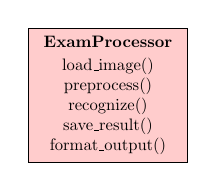
\begin{tikzpicture}[scale=0.6, transform shape]
                \node[draw, rectangle, fill=red!20, minimum width=3cm, minimum height=2cm] {
                    \begin{tabular}{c}
                        \textbf{ExamProcessor} \\[2pt]
                        load\_image() \\
                        preprocess() \\
                        recognize() \\
                        save\_result() \\
                        format\_output()
                    \end{tabular}
                };
            \end{tikzpicture}
        \end{center}

        \column{0.5\textwidth}
        \textbf{改进方案:}
        \begin{center}
            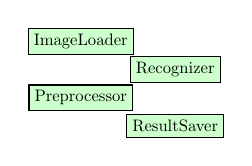
\begin{tikzpicture}[scale=0.6, transform shape]
                \node[draw, rectangle, fill=green!20] (loader) at (-1,0) {ImageLoader};
                \node[draw, rectangle, fill=green!20] (pre) at (-1,-1.2) {Preprocessor};
                \node[draw, rectangle, fill=green!20] (rec) at (1,-0.6) {Recognizer};
                \node[draw, rectangle, fill=green!20] (saver) at (1,-1.8) {ResultSaver};
            \end{tikzpicture}
        \end{center}
    \end{columns}

    \begin{itemize}
        \item SRP使得类更容易理解
        \item 修改只影响少量类
        \item 单元测试更容易编写
    \end{itemize}
\end{frame}

\begin{frame}{开闭原则(OCP)}
    \begin{definition}[开闭原则]
        软件实体应该对扩展开放,对修改关闭。
    \end{definition}

    \textbf{实现方式:}
    \begin{itemize}
        \item 抽象基类 + 具体实现
        \item 策略模式
        \item 依赖注入
        \item 插件架构
    \end{itemize}

    \begin{center}
        \begin{tikzpicture}[scale=0.7, transform shape,
            box/.style={draw, rectangle, minimum width=2.5cm, minimum height=0.7cm}]
            \node[draw, rectangle, dashed] (interface) at (0,0) {<<interface>>\\Recognizer};
            \node[box, fill=blue!15] (choice) at (-2,-1.5) {ChoiceRecognizer};
            \node[box, fill=blue!15] (judge) at (0,-1.5) {JudgeRecognizer};
            \node[box, fill=blue!15] (essay) at (2,-1.5) {EssayRecognizer};
            \node[box, fill=green!15, dashed] (new) at (4,-1.5) {NewRecognizer\\(扩展)};

            \draw[->, thick] (choice) -- (interface);
            \draw[->, thick] (judge) -- (interface);
            \draw[->, thick] (essay) -- (interface);
            \draw[->, thick, dashed] (new) -- (interface);
        \end{tikzpicture}
    \end{center}

    \textbf{OCP的好处:}
    \begin{itemize}
        \item 新功能通过添加新代码实现
        \item 现有代码不会被意外破坏
        \item 系统可维护性大大提高
    \end{itemize}
\end{frame}

\begin{frame}{里氏替换原则(LSP)}
    \begin{definition}[里氏替换原则]
        子类型必须能够替换其基类型,而程序的行为不会改变。
    \end{definition}

    \textbf{关键要求:}
    \begin{itemize}
        \item 子类不改变父类的前置条件(输入)
        \item 子类不强化父类的后置条件(输出)
        \item 子类保持父类的不变性
    \end{itemize}

    \textbf{正确示例:}
    \begin{center}
        \begin{tikzpicture}[scale=0.7, transform shape]
            \node[draw, rectangle, fill=blue!20] (parent) at (0,0) {
                \begin{tabular}{c}
                    \textbf{Recognizer} \\[2pt]
                    recognize(img) -> Result \\
                    preconditions: img不为None \\
                    postconditions: 返回Result对象
                \end{tabular}
            };

            \node[draw, rectangle, fill=green!20] (child) at (0,-2) {
                \begin{tabular}{c}
                    \textbf{OcrRecognizer (子类)} \\[2pt]
                    recognize(img) -> Result \\
                    接受相同输入,产生兼容输出
                \end{tabular}
            };

            \draw[->, thick] (child) -- (parent);
        \end{tikzpicture}
    \end{center}

    \begin{alertblock}{违反LSP的信号}
        \begin{itemize}
            \item 使用instanceof检查子类类型
            \item 需要知道具体子类才能调用
            \item 子类需要覆盖父类方法并抛出异常
        \end{itemize}
    \end{alertblock}
\end{frame}

\begin{frame}{接口隔离原则(ISP)}
    \begin{definition}[接口隔离原则]
        客户端不应该被迫依赖它不使用的方法。应该将大接口拆分为小接口。
    \end{definition}

    \textbf{不好的设计:}
    \begin{center}
        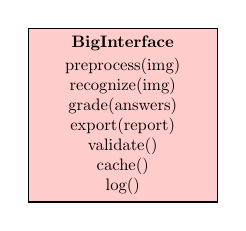
\begin{tikzpicture}[scale=0.6, transform shape]
            \node[draw, rectangle, fill=red!20, minimum width=4cm, minimum height=3cm] {
                \begin{tabular}{c}
                    \textbf{BigInterface} \\[2pt]
                    preprocess(img) \\
                    recognize(img) \\
                    grade(answers) \\
                    export(report) \\
                    validate() \\
                    cache() \\
                    log()
                \end{tabular}
            };
        \end{tikzpicture}
    \end{center}

    \textbf{改进设计:}
    \begin{center}
        \begin{tikzpicture}[scale=0.6, transform shape]
            \node[draw, rectangle, fill=green!15] (p) at (-2,0) {PreprocessorInterface};
            \node[draw, rectangle, fill=green!15] (r) at (0,0) {RecognizerInterface};
            \node[draw, rectangle, fill=green!15] (g) at (2,0) {GraderInterface};

            \node[draw, rectangle, fill=blue!15, minimum width=3cm, minimum height=1.5cm] (impl) at (0,-2) {
                ImageProcessor \\
                实现需要的接口
            };

            \draw[->, thick] (impl) -- (p);
            \draw[->, thick] (impl) -- (r);
            \draw[->, thick] (impl) -- (g);
        \end{tikzpicture}
    \end{center}
\end{frame}

\begin{frame}{依赖倒置原则(DIP)}
    \begin{definition}[依赖倒置原则]
        高层模块不应该依赖低层模块,两者都应该依赖抽象。抽象不应该依赖细节,细节应该依赖抽象。
    \end{definition}

    \textbf{示例对比:}
    \begin{columns}
        \column{0.5\textwidth}
        \textbf{传统方式(违反DIP):}
        \begin{center}
            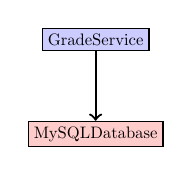
\begin{tikzpicture}[scale=0.6, transform shape]
                \node[draw, rectangle, fill=blue!20] (high) at (0,0) {GradeService};
                \node[draw, rectangle, fill=red!20] (low) at (0,-2) {MySQLDatabase};

                \draw[->, thick] (high) -- (low);
            \end{tikzpicture}
        \end{center}
        \begin{itemize}
            \item 高层依赖低层实现
            \item 更换数据库需要修改高层
            \item 难以测试
        \end{itemize}

        \column{0.5\textwidth}
        \textbf{改进方式(遵循DIP):}
        \begin{center}
            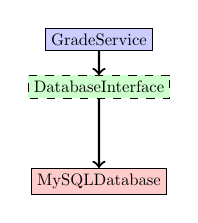
\begin{tikzpicture}[scale=0.6, transform shape]
                \node[draw, rectangle, fill=blue!20] (high) at (0,1) {GradeService};
                \node[draw, rectangle, dashed, fill=green!20] (interface) at (0,0) {DatabaseInterface};
                \node[draw, rectangle, fill=red!20] (low) at (0,-2) {MySQLDatabase};

                \draw[->, thick] (high) -- (interface);
                \draw[->, thick] (interface) -- (low);
            \end{tikzpicture}
        \end{center}
        \begin{itemize}
            \item 依赖抽象接口
            \item 可轻松替换实现
            \item 便于mock测试
        \end{itemize}
    \end{columns}
\end{frame}

\section{设计模式应用}

\begin{frame}{工厂模式}
    \begin{definition}[工厂模式]
        定义一个创建对象的接口,但让子类决定实例化哪个类。工厂方法让类将实例化推迟到子类。
    \end{definition}

    \begin{center}
        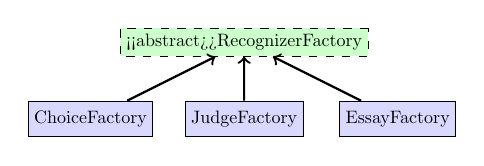
\begin{tikzpicture}[scale=0.65, transform shape,
            box/.style={draw, rectangle, minimum width=2cm, minimum height=0.7cm}]
            \node[draw, rectangle, dashed, fill=green!20] (factory) at (0,0) {<<abstract>>\\RecognizerFactory};
            \node[box, fill=blue!15] (choice) at (-3,-1.5) {ChoiceFactory};
            \node[box, fill=blue!15] (judge) at (0,-1.5) {JudgeFactory};
            \node[box, fill=blue!15] (essay) at (3,-1.5) {EssayFactory};

            \draw[->, thick] (choice) -- (factory);
            \draw[->, thick] (judge) -- (factory);
            \draw[->, thick] (essay) -- (factory);
        \end{tikzpicture}
    \end{center}

    \textbf{使用示例:}
    \begin{center}
        \begin{tikzpicture}[scale=0.7, transform shape]
            \node[draw, rectangle, fill=gray!10, minimum width=6cm, minimum height=2.5cm] {
                \begin{center}
                    \begin{tabular}{l}
                        \texttt{class RecognizerFactory:} \\
                        \texttt{    @staticmethod} \\
                        \texttt{    def create\_recognizer(type\_name):} \\
                        \texttt{        if type\_name == "choice":} \\
                        \texttt{            return ChoiceRecognizer()} \\
                        \texttt{        elif type\_name == "judge":} \\
                        \texttt{            return JudgeRecognizer()} \\
                        \texttt{        ...} \\
                        \\
                        \texttt{\# 使用} \\
                        \texttt{recognizer = RecognizerFactory.create\_recognizer("choice")}
                    \end{tabular}
                \end{center}
            };
        \end{tikzpicture}
    \end{center}
\end{frame}

\begin{frame}{策略模式}
    \begin{definition}[策略模式]
        定义一系列算法,将每个算法封装起来,使它们可以互相替换。策略让算法独立于使用它的客户端。
    \end{definition}

    \begin{center}
        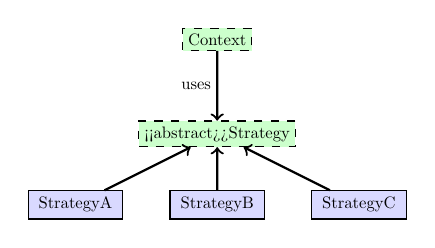
\begin{tikzpicture}[scale=0.6, transform shape,
            box/.style={draw, rectangle, minimum width=2cm, minimum height=0.6cm}]
            \node[draw, rectangle, dashed, fill=green!20] (context) at (0,1) {Context};
            \node[draw, rectangle, dashed, fill=green!20] (strategy) at (0,-1) {<<abstract>>\\Strategy};

            \node[box, fill=blue!15] (s1) at (-3,-2.5) {StrategyA};
            \node[box, fill=blue!15] (s2) at (0,-2.5) {StrategyB};
            \node[box, fill=blue!15] (s3) at (3,-2.5) {StrategyC};

            \draw[->, thick] (context) -- (strategy) node[midway, left] {uses};
            \draw[->, thick] (s1) -- (strategy);
            \draw[->, thick] (s2) -- (strategy);
            \draw[->, thick] (s3) -- (strategy);
        \end{tikzpicture}
    \end{center}

    \textbf{应用场景:}
    \begin{itemize}
        \item 多种识别算法切换
        \item 不同评分策略
        \item 多种输出格式
    \end{itemize}

    \textbf{优点:}
    \begin{itemize}
        \item 算法可以自由切换
        \item 避免使用条件语句
        \item 符合OCP原则
    \end{itemize}
\end{frame}

\begin{frame}{观察者模式}
    \begin{definition}[观察者模式]
        定义对象间的一种一对多依赖关系,当一个对象状态改变时,其所有依赖者都会收到通知并自动更新。
    \end{definition}

    \begin{center}
        \begin{tikzpicture}[scale=0.65, transform shape,
            box/.style={draw, rectangle, minimum width=1.8cm, minimum height=0.6cm}]
            \node[draw, rectangle, fill=yellow!20] (subject) at (0,0) {Subject\\主题};
            \node[box, fill=blue!15] (obs1) at (-3,-2) {Observer1};
            \node[box, fill=blue!15] (obs2) at (0,-2) {Observer2};
            \node[box, fill=blue!15] (obs3) at (3,-2) {Observer3};

            \draw[->, thick] (obs1) -- (subject);
            \draw[->, thick] (obs2) -- (subject);
            \draw[->, thick] (obs3) -- (subject);
            \draw[<->, thick] (subject) -- (obs1) node[midway, right] {notify};
            \draw[<->, thick] (subject) -- (obs2) node[midway, right] {notify};
            \draw[<->, thick] (subject) -- (obs3) node[midway, right] {notify};
        \end{tikzpicture}
    \end{center}

    \textbf{应用场景:}
    \begin{itemize}
        \item 识别完成通知评分模块
        \item 处理进度更新UI
        \item 日志记录事件
    \end{itemize}
\end{frame}

\begin{frame}{装饰器模式}
    \begin{definition}[装饰器模式]
        动态地给一个对象添加额外的职责,比生成子类更灵活。
    \end{definition}

    \begin{center}
        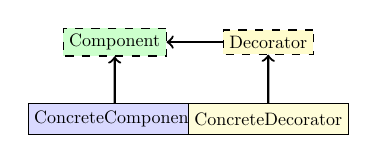
\begin{tikzpicture}[scale=0.65, transform shape,
            box/.style={draw, rectangle, minimum width=2cm, minimum height=0.6cm}]
            \node[draw, rectangle, dashed, fill=green!20] (component) at (0,0) {Component};
            \node[box, fill=blue!15] (concrete) at (0,-1.5) {ConcreteComponent};

            \node[draw, rectangle, dashed, fill=yellow!20] (decorator) at (3,0) {Decorator};
            \node[box, fill=yellow!15] (concreteD) at (3,-1.5) {ConcreteDecorator};

            \draw[->, thick] (concrete) -- (component);
            \draw[->, thick] (concreteD) -- (decorator);
            \draw[->, thick] (decorator) -- (component);
        \end{tikzpicture}
    \end{center}

    \textbf{使用示例:}
    \begin{center}
        \begin{tikzpicture}[scale=0.7, transform shape]
            \node[draw, rectangle, fill=gray!10, minimum width=6cm, minimum height=2.2cm] {
                \begin{center}
                    \begin{tabular}{l}
                        \texttt{class LoggingDecorator(RecognizerInterface):} \\
                        \texttt{    def \_\_init\_\_(self, recognizer):} \\
                        \texttt{        self.\_recognizer = recognizer} \\
                        \\
                        \texttt{    def recognize(self, image):} \\
                        \texttt{        print(f"开始识别")} \\
                        \texttt{        result = self.\_recognizer.recognize(image)} \\
                        \texttt{        print(f"识别完成: \{result\}")} \\
                        \texttt{        return result} \\
                        \\
                        \texttt{\# 使用:添加日志功能} \\
                        \texttt{logged\_rec = LoggingDecorator(basic\_rec)}
                    \end{tabular}
                \end{center}
            };
        \end{tikzpicture}
    \end{center}
\end{frame}

\begin{frame}{模板方法模式}
    \begin{definition}[模板方法模式]
        在抽象类中定义算法的骨架,将某些步骤的具体实现延迟到子类。
    \end{definition}

    \begin{center}
        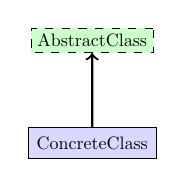
\begin{tikzpicture}[scale=0.65, transform shape,
            box/.style={draw, rectangle, minimum width=2.5cm, minimum height=0.6cm}]
            \node[draw, rectangle, dashed, fill=green!20] (abstract) at (0,0) {AbstractClass};
            \node[box, fill=blue!15] (concrete) at (0,-2) {ConcreteClass};

            \draw[->, thick] (concrete) -- (abstract);
        \end{tikzpicture}
    \end{center}

    \textbf{示例:图像处理流程}
    \begin{center}
        \begin{tikzpicture}[scale=0.7, transform shape]
            \node[draw, rectangle, fill=gray!10, minimum width=7cm, minimum height=2.5cm] {
                \begin{center}
                    \begin{tabular}{l}
                        \texttt{class ImageProcessor:} \\
                        \texttt{    def process(self, image):} \\
                        \texttt{        image = self.load(image)} \\
                        \texttt{        image = self.preprocess(image)} \\
                        \texttt{        image = self.analyze(image)} \\
                        \texttt{        return self.format\_result(image)} \\
                        \\
                        \texttt{    \# 子类实现具体步骤} \\
                        \texttt{    def preprocess(self, image): ...} \\
                        \texttt{    def analyze(self, image): ...}
                    \end{tabular}
                \end{center}
            };
        \end{tikzpicture}
    \end{center}
\end{frame}

\begin{frame}{设计模式总结对比}
    \begin{table}
        \centering
        \small
        \begin{tabular}{p{2cm}p{3cm}p{5cm}}
            \toprule
            \textbf{类型} & \textbf{模式} & \textbf{解决的问题} \\
            \midrule
            \textbf{创建型} & 工厂模式 & 对象创建逻辑复杂,类型需要运行时决定 \\
            & 单例模式 & 需要确保某个类只有一个实例 \\
            & 建造者模式 & 构建复杂对象,参数多,需分步骤构建 \\
            \midrule
            \textbf{结构型} & 适配器模式 & 接口不兼容,需要适配 \\
            & 装饰器模式 & 动态添加功能,不改变原有类 \\
            & 代理模式 & 控制访问,添加代理逻辑 \\
            \midrule
            \textbf{行为型} & 观察者模式 & 一对多通知,状态变化需广播 \\
            & 策略模式 & 算法可互换,需要运行时切换 \\
            & 模板方法 & 算法骨架固定,部分步骤可变 \\
            \bottomrule
        \end{tabular}
    \end{table}

    \begin{alertblock}{使用建议}
        不要为了使用模式而使用模式。只有当问题确实符合模式的应用场景时才使用。
        过度设计比设计不足更糟糕。
    \end{alertblock}
\end{frame}
